\documentclass{beamer}

\mode<presentation> {

% The Beamer class comes with a number of default slide themes
% which change the colors and layouts of slides. Below this is a list
% of all the themes, uncomment each in turn to see what they look like.

%\usetheme{default}
%\usetheme{AnnArbor}
%\usetheme{Antibes}
%\usetheme{Bergen}
%\usetheme{Berkeley}
%\usetheme{Berlin}
%\usetheme{Boadilla}
%\usetheme{CambridgeUS}
%\usetheme{Copenhagen}
%\usetheme{Darmstadt}
%\usetheme{Dresden}
\usetheme{Frankfurt}
%\usetheme{Goettingen}
%\usetheme{Hannover}
%\usetheme{Ilmenau}
%\usetheme{JuanLesPins}
%\usetheme{Luebeck}
%\usetheme{Madrid}
%\usetheme{Malmoe}
%\usetheme{Marburg}
%\usetheme{Montpellier}
%\usetheme{PaloAlto}
%\usetheme{Pittsburgh}
%\usetheme{Rochester}
%\usetheme{Singapore}
%\usetheme{Szeged}
%\usetheme{Warsaw}

% As well as themes, the Beamer class has a number of color themes
% for any slide theme. Uncomment each of these in turn to see how it
% changes the colors of your current slide theme.

%\usecolortheme{albatross}
%\usecolortheme{beaver}
%\usecolortheme{beetle}
\usecolortheme{crane}
%\usecolortheme{dolphin}
%\usecolortheme{dove}
%\usecolortheme{fly}
%\usecolortheme{lily}
%\usecolortheme{orchid}
%\usecolortheme{rose}
%\usecolortheme{seagull}
%\usecolortheme{seahorse}
%\usecolortheme{whale}
%\usecolortheme{wolverine}

%\setbeamertemplate{footline} % To remove the footer line in all slides uncomment this line
%\setbeamertemplate{footline}[page number] % To replace the footer line in all slides with a simple slide count uncomment this line

%\setbeamertemplate{navigation symbols}{} % To remove the navigation symbols from the bottom of all slides uncomment this line
}

\usepackage{extpfeil}
\usepackage{extarrows} %Allows long equation signs
\usepackage{graphicx} % Allows including images
\usepackage{booktabs} % Allows the use of \toprule, \midrule and \bottomrule in tables
\usepackage{physics}
\usepackage{tikz}
\usepackage{cite}
%花体字母
\usepackage{amsthm,amsmath,amssymb}
\usepackage{mathrsfs}
\usepackage{dutchcal}
\usepackage{circuitikz}

%----------------------------------------------------------------------------------------
%	TITLE PAGE
%----------------------------------------------------------------------------------------

\title[VP260 RC]{VP260 Recitation Class} % The short title appears at the bottom of every slide, the full title is only on the title page

\author{VP260 TA Group} % Your name
\institute[UM-SJTU JI] % Your institution as it will appear on the bottom of every slide, may be shorthand to save space
{
    University of Michigan - Shanghai Jiao Tong University Joint Institute\\% Your institution for the title page
\medskip
}
\date{\today} % Date, can be changed to a custom date

\begin{document}

\begin{frame}
    \titlepage % Print the title page as the first slide
\end{frame}

%----------------------------------------------------------------------------------------
%	 SECTION 1
%----------------------------------------------------------------------------------------

\section{Vector Calculus} % Section title slide, unnumbered

\begin{frame}{Stoke's formula}
	\begin{beamerboxesrounded}{Foundamental theorem for gradients}
		\begin{equation}
			\int_{\vb{a}}^{\vb{b}} (\grad f) \vdot \dd{\vb*{l}} = f(\vb{b}) - f(\vb{a})
		\end{equation}
	\end{beamerboxesrounded}
	
	\begin{beamerboxesrounded}{Divergence theorem}
		\begin{equation}
			\int_V (\div \vb{v}) \dd{\tau} = \oint_{\partial V} \vb{v} \vdot \dd{\vb*{A}}
		\end{equation}
	\end{beamerboxesrounded}

	\begin{beamerboxesrounded}{Stoke's theorem}
		\begin{equation}
			\int_S (\curl \vb{v}) \vdot \dd{\vb{A}} = \oint_{\partial S} \vb{v} \vdot \dd{\vb{l}}
		\end{equation}
	\end{beamerboxesrounded}
\end{frame}

\section{Electrostatics}

\begin{frame}{Coulomb Force}	
	\begin{beamerboxesrounded}{Coulomb Force}
		\begin{equation}
			\vec{F} = \frac{1}{4\pi\epsilon_0} \frac{\abs{q_1 q_2}}{r^2} \vu{r}
		\end{equation}	
    \end{beamerboxesrounded}

	\begin{itemize}
		\item permittivity of vacuum: $\epsilon_0 = 8.85 \times 10^{-12} \  C^2/(N \cdot m^2)$;
        \item The direction of $\vu{r}$ is decided by charges;
        \item Superposition principle.
	\end{itemize}
\end{frame}


\begin{frame}{Electric Field}	
	\begin{beamerboxesrounded}[shadow=true]{Electric Field}
        \begin{equation}
			\vec{E} = \frac{\vec{F}}{q_0}
		\end{equation}
    \end{beamerboxesrounded}
	
	\begin{itemize}
		\item Only valid when $q_0$ is a point charge.
		\item Electric field is a vector field in space.
		\item "real" physical entity
        \item unit: $V/m$ or $N/C$
        \item $\va{E}$ is tangential to the field line.
		\item Field lines only intersect at point charges.
		\item Density of field line represents the magnitude of $\va{E}$.
	\end{itemize}
\end{frame}


\begin{frame}{Electric Potential}
    We can prove that $\oint_l \va{E} \vdot \dd{\va{s}} = 0$ and $\curl{\va{E}} = 0$.

    \begin{block}{Electric potential}
        \begin{equation}
            V(\va{r}) = -\int_O^{\va{r}} \va{E} \vdot \dd{\va{l}}
        \end{equation}

        \begin{itemize}
            \item Here, point O is zero reference. We use infinity as reference point usually.
            \item Unit: [V]olt
        \end{itemize}	
    \end{block}

    \begin{block}{Toolbox for calculating potential}
        \begin{itemize}
            \item $V(\va{r}) = -\int_O^{\va{r}} \va{E} \vdot \dd{\va{l}}$;
            \item Add up contributions from small charges dq regarded as point charges;
            \item Solve equation $- \laplacian{V} = \frac{\rho}{\epsilon_0}$ with boundary condition.
        \end{itemize}
    \end{block}
\end{frame}


\begin{frame}{Gauss' Law}
	\begin{beamerboxesrounded}{Electric flux}
		\begin{equation}
			\Phi_E = \int_{S} \va{E} \vdot \dd{\va{A}}
		\end{equation}
	\end{beamerboxesrounded}
	\vspace{1em}
	\begin{beamerboxesrounded}{Gauss' law}
		\begin{equation}
			\oint_{S} \va{E} \cdot \dd{\va{A}} = \frac{q_{enc}}{\epsilon_0}
		\end{equation}
		\begin{equation}
			\div \va{E} = \frac{\rho(\vec{r})}{\epsilon_0}
		\end{equation}
	\end{beamerboxesrounded}
	\begin{itemize}
		\item The $q_{enc}$ is the total charge enclosed in the surface.
	\end{itemize}
\end{frame}


\begin{frame}{Potential energy}
    Move a test charge $q$ from point $\va{a}$ to $\va{b}$, the minimum work is,
    \begin{equation}
        W = \int_{\vb{a}}^{\vb{b}} \va{F} \vdot \dd{\va{l}} = -q \int_{\vb{a}}^{\vb{b}} \va{E} \vdot \dd{\va{l}} = q \cdot (V(\va{a}) - V(\va{b}))
    \end{equation}

    \begin{block}{Potential energy}
        \begin{equation}
            U(\va{r}) = q \cdot V(\va{r})
        \end{equation}
    \end{block}

    \begin{itemize}
        \item The minimum work for moving a test charge $q$ from point $\va{a}$ to $\va{b}$ is $U(\va{a}) - U(\va{b})$.
    \end{itemize}
\end{frame}


\begin{frame}{Configuration Energy}
    Discrete distribution,
    \begin{equation}
        U_{conf} = \frac{1}{8 \pi \epsilon_0} \sum_{i} \sum_{j, i \neq j} \frac{q_i q_j}{r_{ij}} = \frac{1}{2} \sum_{i} q_i V(\va{r_i}).
    \end{equation}

    Continuous distribution,
    \begin{equation}
        U_{conf} = \frac{1}{2} \int_{\Omega} \rho V \dd{\tau} = \frac{\epsilon_0}{2} \left( \oint_{\Sigma} V \va{E} \vdot \dd{\va{A}} + \int_{\Omega} E^2 \dd{\tau} \right).
    \end{equation}

    For the whole space,
    \begin{equation}
        U_{conf} = \frac{\epsilon_0}{2} \int_{\mathbb{R}^3} E^2 \dd{\tau}.
    \end{equation}
\end{frame}


\begin{frame}{Conductor}
    \begin{itemize}
        \item Electric field lines is perpendicular to equipotential surfaces;
        \item The surface of a conductor is equipotential (electrostatic).
    \end{itemize}
    \vspace{1em}
    \begin{beamerboxesrounded}[shadow=true]{Properties of Conductors}
        \begin{itemize}
            \item $\va{E} = 0$ \textbf{everywhere} inside a conductor;
            \item Any excess charge placed on a conductor resides entirely on its surface;
            \item Any conductor is equipotential.
        \end{itemize}
    \end{beamerboxesrounded}
\end{frame}


\begin{frame}{Poisson's Equation}
    \begin{block}{Recall: (Gauss' Law)}
        \begin{equation}
            \div{\va{E}} = \frac{\rho}{\epsilon_0}
        \end{equation}  
        \text{Since $\va{E} = -\grad{V}$, then we have:}
        \begin{equation}
            \div(-\grad{V}) = -\laplacian{V} = \frac{\rho}{\epsilon_0}
        \end{equation}
    \end{block}

    \begin{block}{Poisson's Equation (PDE)}
        \begin{equation}
            - \laplacian{V} = \frac{\rho}{\epsilon_0}
        \end{equation}
    \end{block}
\end{frame}


\begin{frame}{Method of Image}
    Poisson's equation provides us an efficient and systematic way to solve the electric potential distribution in space.
    However, it is not easy to solve a PDE. Here, we will briefly introduce:
    \vspace{.5em}
    
    \begin{beamerboxesrounded}[shadow=true]{Method of Images}
        Add mirror images \textbf{outside} the original domain, to satisfy the boundary conditions.
    \end{beamerboxesrounded}
    \begin{block}{Uniqueness theory}
        The electric potential inside a certain is \textbf{uniquely} determined, if:
        \begin{itemize}
            \item Charge density $\rho$ throughout the domain $\Omega$ is known
            \item The electric potential distribution at the boundaries is known
        \end{itemize}
    \end{block}
\end{frame}

\begin{frame}{Summary for Electrostatics}
    \begin{figure}[htbp]
        \centering
        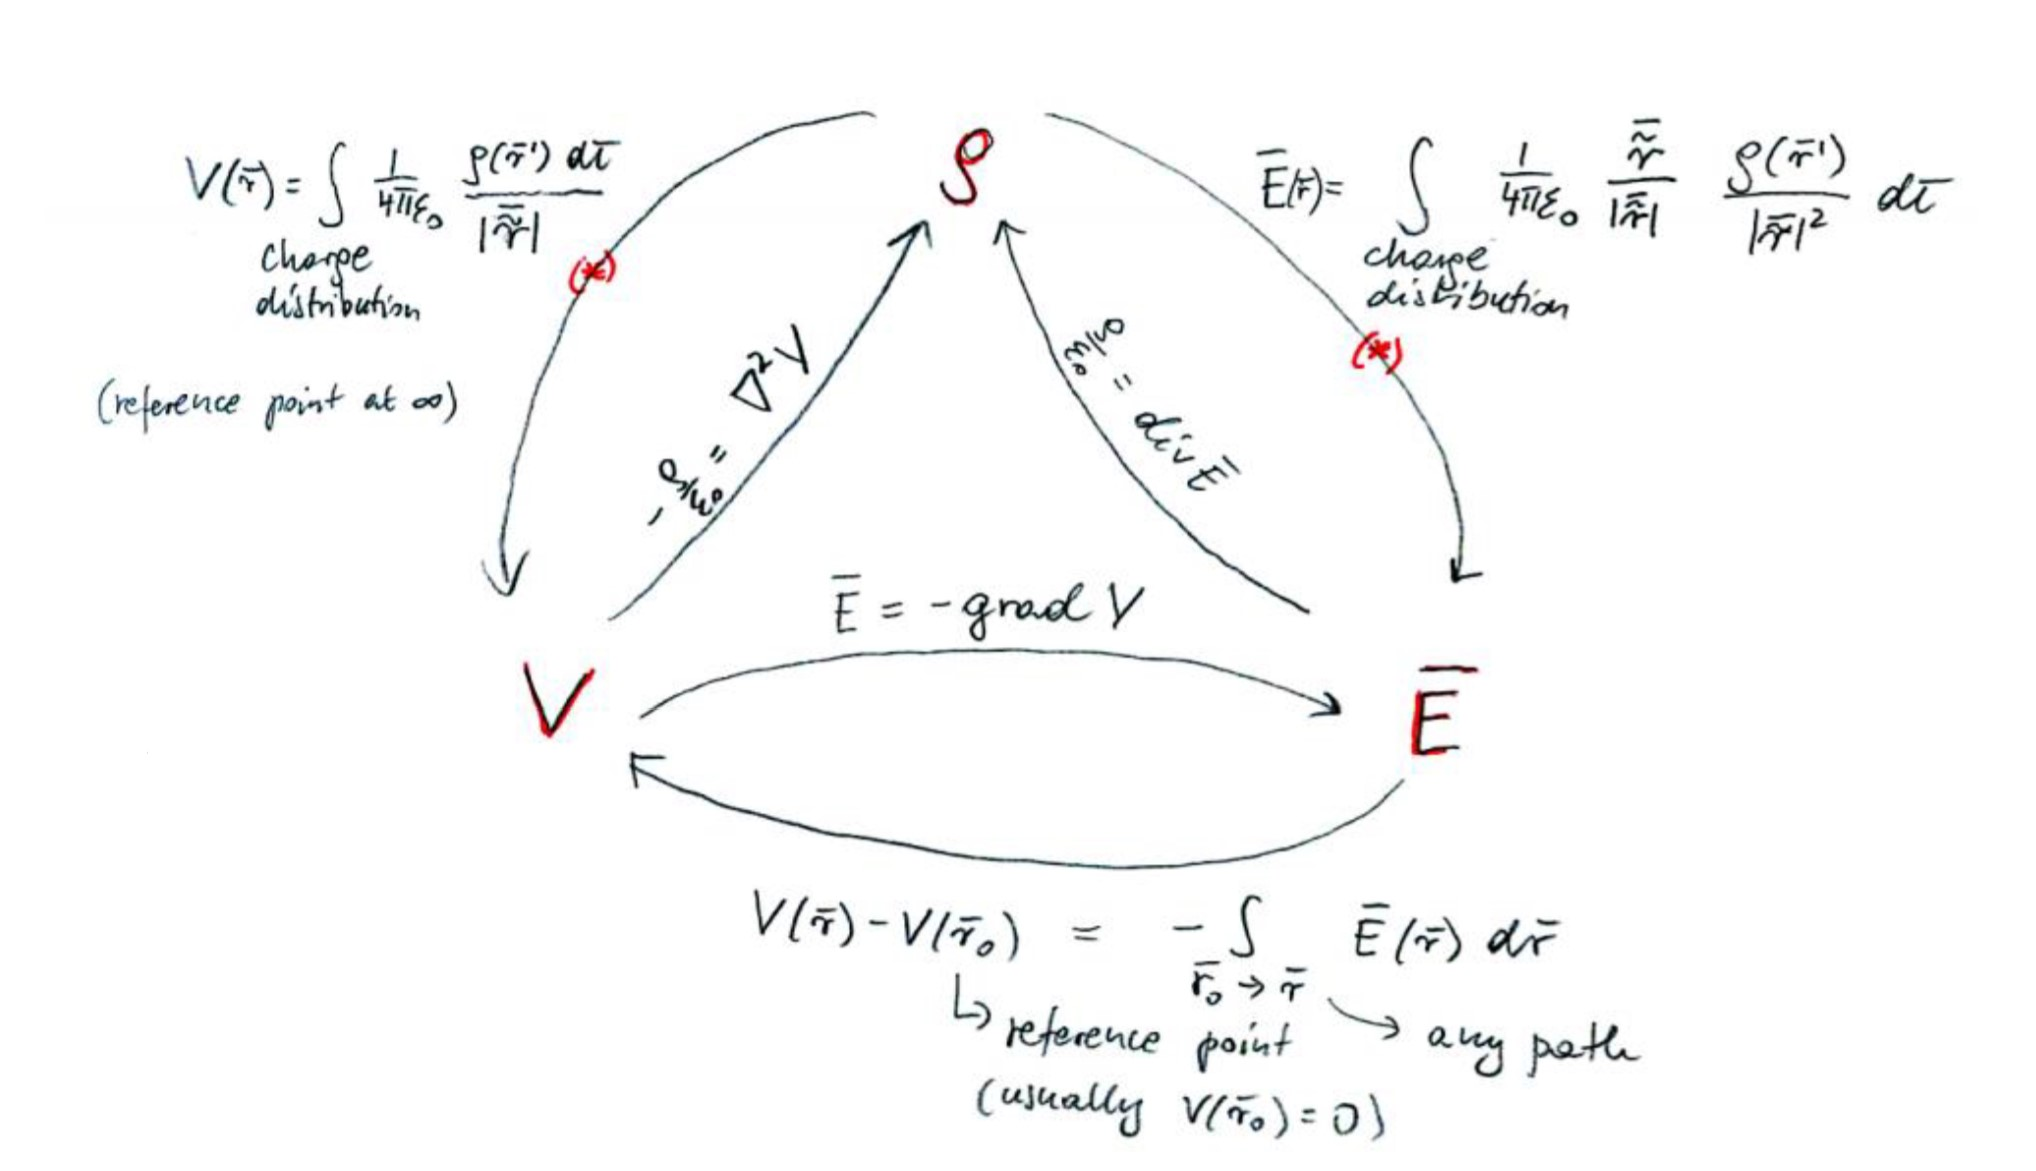
\includegraphics[width=\textwidth]{images/elec.jpg}
    \end{figure}
\end{frame}

%------------------------------------------------

\section{DC Circuit}

\begin{frame}{Capacitor \& Capacitance}
    \begin{beamerboxesrounded}[shadow=true]{Capcitance}
        \begin{equation}
            C = \frac{Q}{V_{ab}}
        \end{equation}
    \end{beamerboxesrounded}
    \begin{itemize}
        \item Unit: $1F = 1C/1V$
        \item $V_{ab} = V_a - V_b$
    \end{itemize}

    \begin{beamerboxesrounded}[shadow = true]{Energy}
        \begin{equation}
            U = W = \frac{Q^2}{2C} = \frac{1}{2} CV^2 
        \end{equation}
    \end{beamerboxesrounded}

    \begin{block}{Energy density}
        \begin{equation}
            u = \frac{1}{2} \epsilon_0 E^2
        \end{equation}
    \end{block}     
\end{frame}


\begin{frame}{Dielectrics}
    \begin{itemize}
        \item Relative permittivity: $ \epsilon_r $
        \item Absolute permittivity: $ \epsilon = \epsilon_r \epsilon_0 $
    \end{itemize}
    \vfill
    \begin{beamerboxesrounded}[shadow=true]{Formulas with dielectrics}
        \begin{equation}
            \left\{
                \begin{array}{ll}
                    \vspace{.5em}
                   & V = \frac{V_0}{\epsilon_r} \\ \vspace{.5em}
                   & E = \frac{E_0}{\epsilon_r} = \frac{\sigma}{\epsilon} \\ \vspace{.5em}
                   & C = \epsilon \frac{A}{d} \\\vspace{.5em}
                   & u = \frac{1}{2} \epsilon E^2
                \end{array}
            \right.
        \end{equation}
    \end{beamerboxesrounded}    
\end{frame}

\begin{frame}{Electric Current}
    \begin{beamerboxesrounded}[shadow=true]{Current density}
        \begin{equation}
            \begin{array}{llll}
               & \va*{J} &=& qn\va*{v_d} \vspace{.6em}\\
               & \abs*{\va*{J}} &=& \frac{I}{A}
            \end{array}
        \end{equation}
    \end{beamerboxesrounded}
    \vfill
    \begin{beamerboxesrounded}[shadow=true]{Ohm's law (microscopic form)}
        \begin{equation}
            \begin{split}
                \va*{J} &= \sigma \va*{E} \\
                \va*{J} &= \frac{\va*{E}}{\rho}
            \end{split}
        \end{equation}
    \end{beamerboxesrounded}
\end{frame}

\begin{frame}{Kirchhoff's Rule}
    \begin{block}{Kirchhoff's rule}
        \begin{itemize}
            \item Junction rule (KCL):
                \begin{equation}
                    \sum_k I_k = 0
                \end{equation}
                where $I_k$ represents a current flows into the junction.
            \item Loop rule (KVL):
                \begin{equation}
                    \sum_k V_k = 0
                \end{equation}
                where $V_k$ represents the voltage across the element in a loop
        \end{itemize}.
    \end{block}
\end{frame}

\begin{frame}{Direct Current RC Circuits}
    \begin{columns}
        \begin{column}{.5\linewidth}
            \begin{block}{Charging}
                \begin{center}
                    \begin{circuitikz}
                        \draw (0,0) to[battery1=$\epsilon$] (4,0) -- (4,2) to[R=$R$](2,2) -- (1.5,2) to[C=$C$] (0,2) -- (0,0);
                    \end{circuitikz}
                \end{center}
            \end{block}
        \end{column}

        \begin{column}{.5\linewidth}
            \begin{block}{Discharging}
                \begin{center}
                    \begin{circuitikz}
                        \draw (0,0) to[R=$R$] (4,0) -- (4,2) to[C=$C$] (0,2) -- (0,0);
                    \end{circuitikz}
                \end{center}
            \end{block}
        \end{column}
    \end{columns}
\end{frame}


\section{Magnetic field}

\begin{frame}{Magnetic Force}
    \begin{block}{Lorentz force}
        \begin{equation}
            \va{F} = q (\va{v} \crossproduct \va{B})
        \end{equation}
    \end{block}
    \begin{itemize}
        \item Magnetic forces do no work.
    \end{itemize}
    \vfill
    \begin{block}{Ampere's force}
        The magnetic force on a segment of current-carrying wire is,
        \begin{equation}
            \va{F} = \int I (\dd{\va{l} \crossproduct \va{B}})
        \end{equation}
    \end{block}
\end{frame}


\begin{frame}{Magnetic Fluxa and Gauss' Law}
    \begin{block}{Magnetic flux}
        \begin{equation}
            \Phi_B = \int_\Sigma \va{B} \vdot \dd{\va{A}}
        \end{equation}
    \end{block}
    \begin{itemize}
        \item Unit: Weber [Wb]
    \end{itemize}
    \vfill
    \begin{block}{Gauss' law for the magnetic field}
        For any closed surface $\Sigma$,
        \begin{equation}
            \Phi_B = \oint_\Sigma \va{B} \vdot \dd{\va{A}} = 0
        \end{equation}
        Hence,
        \begin{equation}
            \div{\va{B}} = 0
        \end{equation}
    \end{block}
\end{frame}



%----------------------------------------------------------------------------------------
%	 Section 2
%----------------------------------------------------------------------------------------

\section{Exercise}


%----------------------------------------------------------------------------------------
%	 CLOSING/SUPPLEMENTARY SLIDES
%----------------------------------------------------------------------------------------

\begin{frame}
    \begin{center}
        \LARGE\bf LALALA
    \end{center}
	
\end{frame}


\section{Appendix}

%----------------------------------------------------------------------------------------

\begin{frame}{\bf References}
	\nocite{*} % Display all references regardless of if they were cited
	\bibliography{example.bib}
	\bibliographystyle{plain}
\end{frame}

\end{document}

